
\chapter{La tecnologia Blockchain}\makeatletter\def\@currentlabel{1}\makeatother
\label{cap1}
\lhead{\textbf{CAPITOLO 1.}  \textit{LA TECNOLOGIA BLOCKCHAIN}}
\section{Che cosa si intende per Blockchain?}\label{Capitolo1.1}
La Blockchain è una tecnologia che si basa su due concetti dell'informatica presenti da diversi decenni: la crittografia e i sistemi distribuiti.
Prima di approfondire il funzionamento della tecnologia Blockchain, introduciamo brevemente questi due concetti caratteristici:

\begin{itemize}
    \item Citando \cite{crittografia_definizione}:“La \textit{crittografia} è la branca della crittologia che tratta i metodi per rendere un messaggio non comprensibile/intelligibile a persone non autorizzate a leggerlo, garantendo così, in chiave moderna, il requisito di confidenzialità o riservatezza tipico della sicurezza informatica. [...]”;
    
    \item Citando \cite{sistemi_distribuiti}:“[...]Un \textit{sistema distribuito} è una collezione di computer indipendenti che appare ai propri utenti come un singolo sistema coerente. [...]”.Esso consiste di una serie di computer autonomi, connessi tra loro attraverso una rete e un middleware\footnote{Insieme di programmi informatici che fungono da intermediazione tra applicazioni o componenti software.} di distribuzione centrale. Il quale consente ai computer di coordinare le loro attività e di condividere le risorse di sistema.
    
\end{itemize}

Il genio di Satoshi Nakamoto\footnote{Pseudonimo del creatore (o dei creatori) di Bitcoin} è stato il primo a combinare queste due nozioni, in una forma mai vista prima d'ora, il tutto definito nel whitepaper\footnote{Documento che include uno schema di un problema che il progetto sta cercando di risolvere, la soluzione a quel problema, nonché una descrizione dettagliata del loro prodotto, della sua architettura e della sua interazione con gli utenti.} di Bitcoin(Da \cite{bitcoin_definizione}:“[...] è una criptovaluta e un sistema di pagamento valutario internazionale [...]”.Descritta per la prima volta in \cite{bitcoin}. Essa è basata sulla tecnologia che descriveremo in questo capitolo.).
Una prima definizione che possiamo dare alla tecnologia Blockchain è quella di essere una struttura dati condivisa, sicura e immutabile; il modo per cui possiede tutte queste caratteristiche verrà spiegato, in dettaglio, nel paragrafo successivo.


\section{Come funziona la tecnologia Blockchain?} \label{1.2}
Per poter capire al meglio il funzionamento della Blockchain, è doveroso analizzare il concetto di \textit{ledger distribuito o decentralizzato} (DL).

Un \textit{Distributed Ledger} è un \textit{record}\footnote{Un record è un tipo di dato strutturato che comprende diversi elementi (detti campi o membri) di tipo eterogeneo} condiviso e sincronizzato consensualmente tra più siti, istituzioni o aree geografiche, accessibile da più persone. Esso non ammette amministrazione centralizzata o archiviazione centralizzata dei dati, il tutto viene gestito da una rete distribuita di computer, tipicamente di tipo Peer-to-Peer\footnote{ È un'architettura di rete detta “paritaria” in cui i nodi fungono sia da client che da server. Questi nodi sono definiti equivalenti o paritari(peer).}(P2P).

Questi DL vengono realizzati grazie alla \textit{Decentralized Ledger Tecnology} (DLT), quest'ultima ha come primario obiettivo quello di realizzare un grande network formato da diversi partecipanti, ognuno  dei quali è chiamato a gestire un nodo della rete. Ciascun nodo è autorizzato ad aggiornare i DL in modo indipendente ma sempre sotto il controllo consensuale degli altri nodi. Il modo con cui si raggiunge questo “accordo” consensuale e la struttura dei DL sono solo alcune delle caratteristiche che connotano una DLT rispetto ad un'altra.

L'idea della prima Blockchain (Bitcoin) è quella di realizzare un network che strutturi i DL come una catena di blocchi contenenti transazioni. Questa catena non è altro che un database generale distribuito facente parte di ogni nodo della rete che, a sua volta, implementa le caratteristiche di cui sopra descritte per una DLT.

Analizzeremo ora, nel dettaglio, il contenuto che permette il funzionamento di questa tecnologia, tenendo in considerazione che i meccanismi analizzati verteranno principalmente sulle caratteristiche di Blockchain utilizzatrici dell' \textit{algoritmo di consenso}\footnote{Da un articolo dell'accademy di Binance \cite{algoritmo_consenso}:“Un algoritmo di consenso è un meccanismo che permette a utenti o dispositivi di coordinarsi in un contesto distribuito. Deve garantire che tutti gli agenti nel sistema possano concordare su una singola fonte di verità, anche se alcuni agenti falliscono.[...]”} \textit{Proof-Of-Work} (PoW)\footnote{PoW è il padre degli algoritmi di consenso,esso viene utilizzato dalle più famose reti di criptovalute.}, come Bitcoin.

\subsection{La struttura del blocco}\label{struttura_blocco}
Per iniziare, diamo una panoramica generale della struttura del singolo blocco di una Blockchain.
Un blocco è suddiviso in due parti distinte: L'\textit{header} e il \textit{body}.
L'\textit{header} del blocco, come mostrato in figura \ref{struttura_blocco_img}, è composto da sei campi che hanno il compito di gestire il blocco stesso:
\begin{figure}[h]
    \centering
    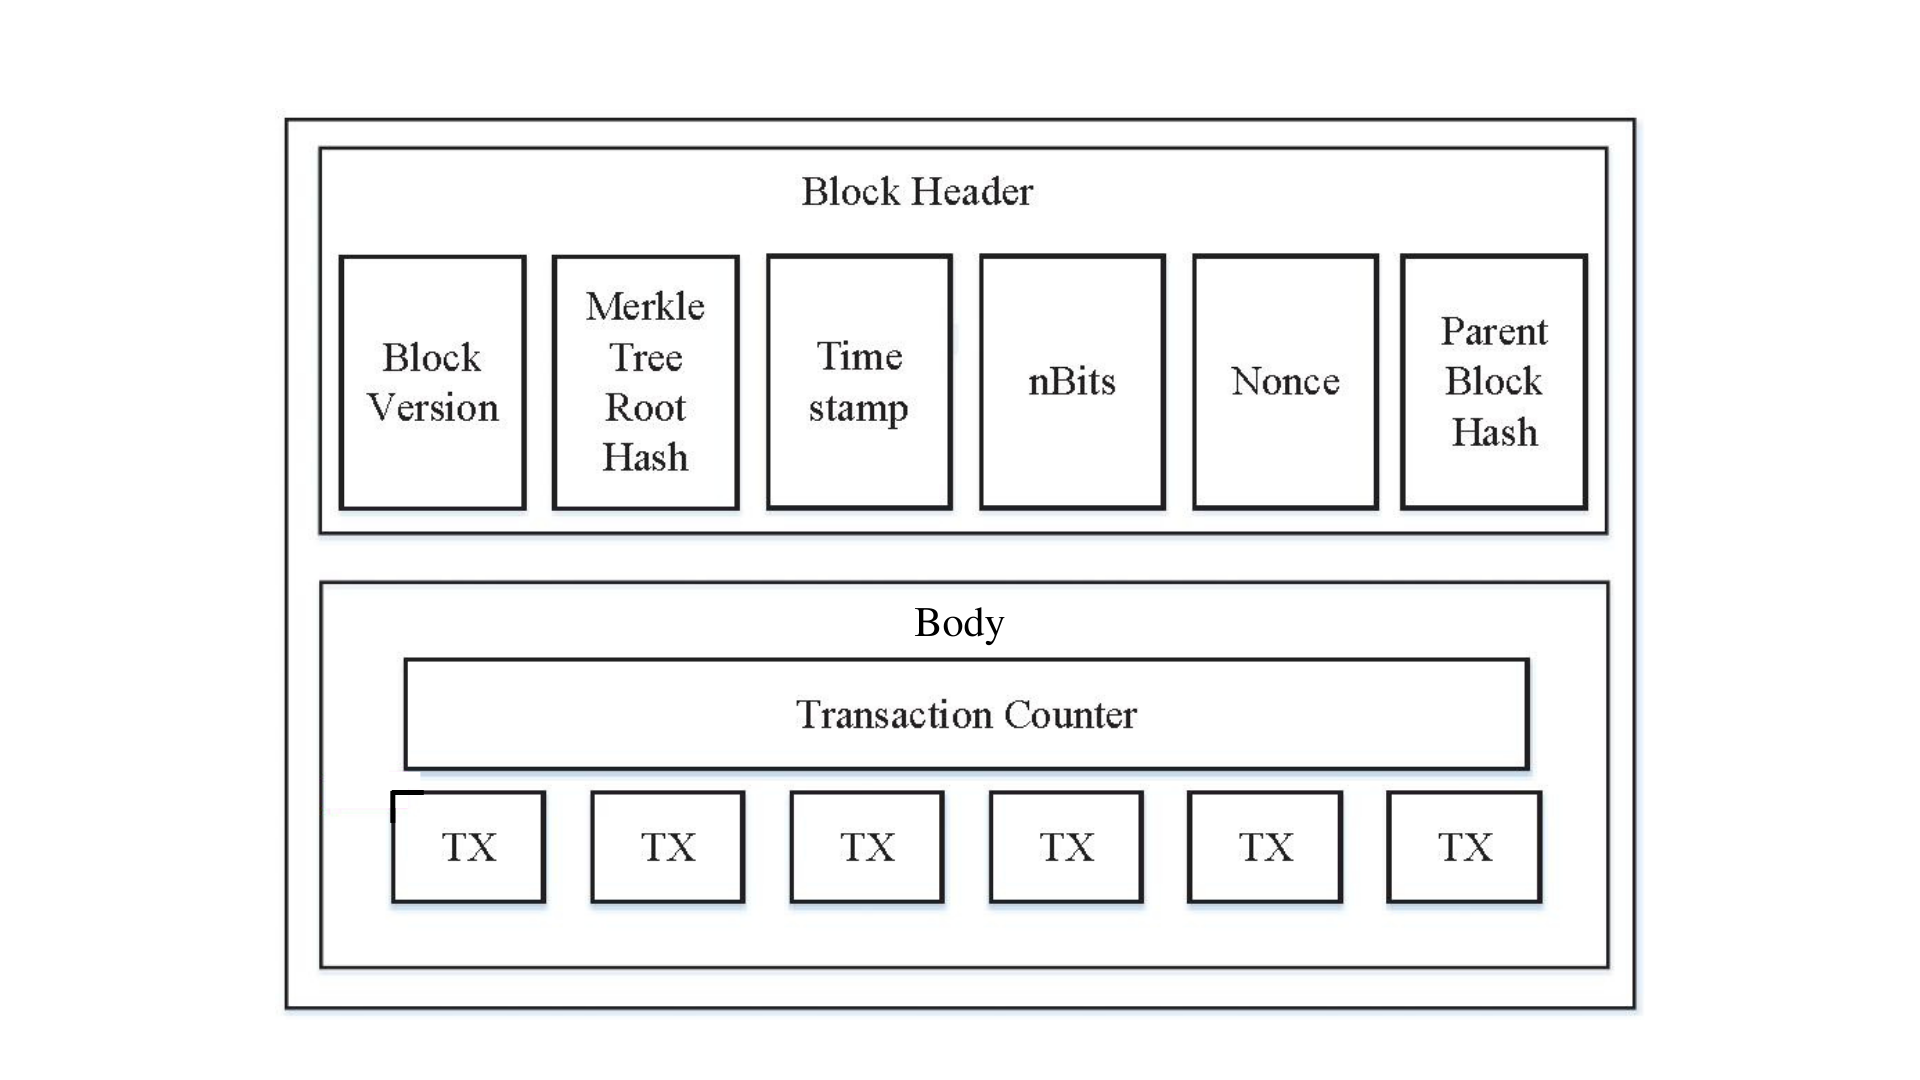
\includegraphics[width=14cm,height=7cm]{Immagini/Struttura_blocco.png}
    \caption[Struttura di un blocco della catena]{Struttura di un blocco della catena.}
    \label{struttura_blocco_img}
\end{figure}
\begin{itemize}
    \item La \textit{versione}, la quale indica le regole di \textit{validazione del blocco}\footnote{L'operazione di validazione del blocco è l'elemento essenziale della Blockchain, permette l'aggiunta del blocco alla fine della catena dopo una serie di verifiche e controlli che verranno approfonditi in (\ref{mining}).} da rispettare. Esse dipendono dalla versione del software che viene utilizzato per una specifica Blockchain;

    \item Il \textit{Parent Block Hash}(o \textit{Previous Hash}) è un valore di 256 bit riferito al blocco precedente della catena. Se il valore hash del blocco precedente a cui è riferito cambia, anche il PreviousHash cambierà, innescando, così, una reazione a catena di aggiornamento di identità tra tutti i blocchi successivi al blocco modificato. Verrà approfondito in (\ref{hashing});
    \item Il \textit{Merkle Tree Root Hash} è una struttura dati con diversi use-case. Uno dei principali è quello di garantire l'integrità dei dati usufruendo dell'hashing. Verrà approfondito in (\ref{Merkle_Tree});
    \item Il \textit{timestamp}, letteralmente “marca temporale”, rappresenta un preciso istante, con lo scopo di accertare l’effettivo avvenimento di un determinato evento;
    \item Il campo \textit{Bits}(o \textit{difficulty target}) è la soglia \textit{target} calcolata dall'algoritmo Proof-Of-Work di un hash di blocco valido;
    \item Il campo \textit{Nonce} è un valore in byte, aggiunto al blocco e ricalcolato tramite \textit{rehashing}\footnote{Procedura che identifica delle operazioni di \textit{hashing} ripetute nel tempo.} in maniera tale che quest'ultimo rispetti dei criteri per la validazione del blocco. Questa operazione necessita di una grande potenza di calcolo; si tratta del famoso \textit{mining}, approfondito in (\ref{mining}).
\end{itemize}

Il \textit{body} del blocco, invece, è composto da un \textit{contatore di transazioni} e dalle transazioni vere e proprie (indicate come “TX” nella figura \ref{struttura_blocco}). Queste transazioni devono essere \textit{verificate}\footnote{La verifica di una transazione consiste nella conferma dei dettagli della transazione, inclusi il tempo della transazione, l’importo e i partecipanti.}. Il funzionamento e la logica delle transazioni verrà approfondito in (\ref{transazioni}).
\subsection{L'hashing per il collegamento dei blocchi} \label{hashing}
\begin{figure}[h]
    \centering
    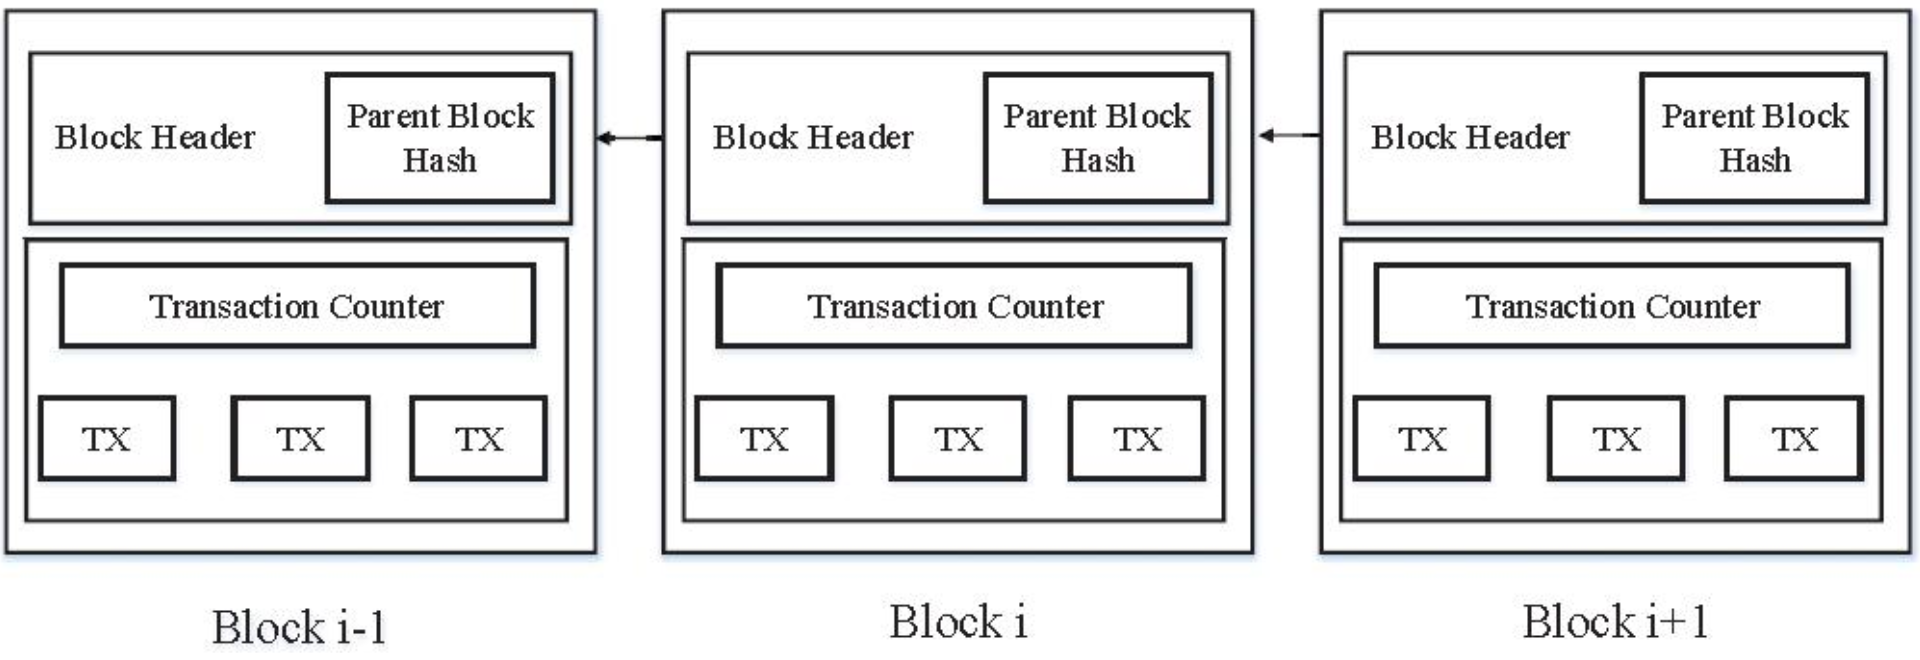
\includegraphics[width=12.5cm,height=5cm]{Immagini/Catena.png}
    \caption[Schema base di una catena di blocchi]{Schema base di una catena di blocchi (Blockchain).}
    \label{catena}
\end{figure}
Come accennato, la Blockchain è una struttura dati formata da una serie di blocchi collegati tra di loro(un esempio di schema base viene mostrato in figura \ref{catena}).
I nuovi blocchi si formano quando i partecipanti della rete creano nuovi dati o aggiornano quelli già esistenti. Questi blocchi memorizzano dei dati crittografati e dotati di un ID\footnote{Abbreviazione di “Identificativo”.} univoco, chiamato Hash.
Nella Blockchain l’hash è il collante che tiene insieme i blocchi, creando, a tutti gli effetti, una \textit{catena di blocchi}. L'hash rende questa catena a prova di manomissioni garantendo l'integrità e l'autenticità dei dati presenti in ogni singolo blocco. In questo paragrafo introdurremo il funzionamento dell'hashing in generale e l'utilizzo specifico per la tecnologia Blockchain.

Per hashing si intende il processo nel quale una qualsiasi chiave k viene inserita in una \textit{funzione di hash} h in modo da ottenere un intero\footnote{In informatica, un intero viene definito come un tipo di dato utilizzato per rappresentare numeri reali che non hanno valori frazionari.} h(k). La coppia chiave-valore \lstinline|<k,v>| viene memorizzata in un vettore (detto \textit{tabella di hash}) nella posizione h(k).
Una funzione hash è definita come:

\begin{equation*}
    h:U \rightarrow  \{0,1,...,m-1\} , dove:
\end{equation*}

\begin{itemize}
    \item \textit{h}, come anticipato, è la funzione di hash;
    \item \textit{U} è l'insieme Universo (insieme delle possibili chiavi);
    \item \textit{m} $\in \mathbb{N}$ è la dimensione del vettore T;
    \item \textit{T} è la tabella di hash nel quale vengono memorizzate le coppie chiave-valore.Un esempio lo si mostra in \ref{tabella_hash}.
\end{itemize}
\begin{figure} [h]
    \centering
    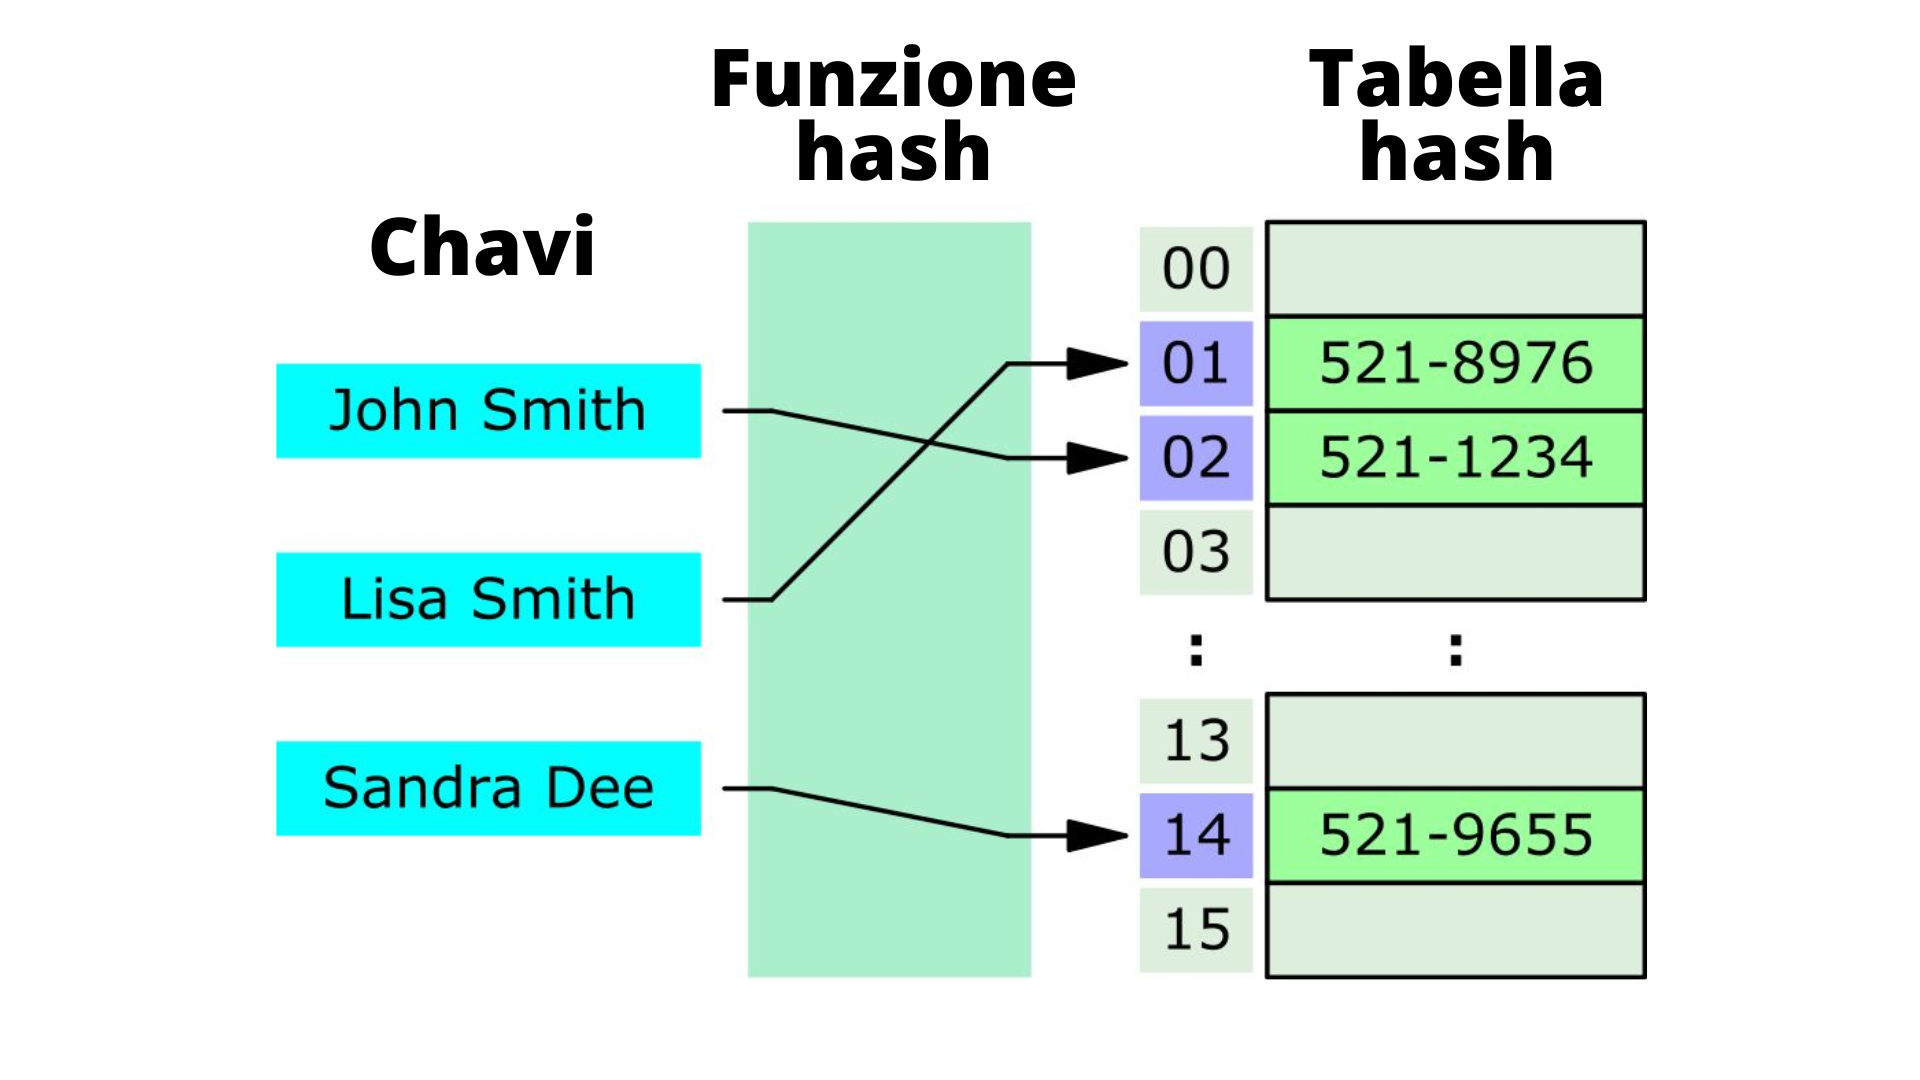
\includegraphics[width=12cm,height=5cm]{Immagini/Chavi.png}
    \caption[Esempio di tabella hash]{Esempio di tabella hash.}
    \label{tabella_hash}
\end{figure}

Nell'ambito Blockchain si utilizzano le \textit{funzioni crittografiche di hash}, le quali, non sono altro che una categoria speciale delle funzioni di hash classiche. Queste particolari funzioni devono:

\begin{itemize}
    \item essere \textit{deterministiche} (cioè ogni messaggio possiede il sempre lo stesso hash);
    \item rendere univoco il valore di hash per ogni input;
    \item rendere molto difficile poter generare un messaggio da un dato valore di hash;
    \item essere veloci nel calcolare il valore di hash.
\end{itemize}.  
Queste caratteristiche peculiari delle \textit{funzioni crittografiche di hash} le rendono particolarmente adatte per garantire l'integrità, l'autenticità e la sicurezza dei dati.

Applicate al contesto Blockchain, l'hash è ciò che conferisce l'unicità al singolo blocco. Ogni blocco della catena dipende dal precedente, poiché, nel pacchetto di dati di ognuno di essi, è incluso l’hash del blocco antecedente ad esso; ciò comporta l'alterazione di tutti i blocchi successivi, ogniqualvolta, un dato blocco viene modificato dopo la registrazione iniziale dei dati per quest'ultimo.
Come anticipato in (\ref{struttura_blocco}), ogni blocco possiede un \textit{timestamp}, che, esattamente come gli altri componenti, influenza inevitabilmente il valore hash del blocco e, come si dice in \cite{bitcoin}:“[...] prova che i dati devono essere esistiti in quella determinata data, dal momento che sono finiti nell'hash.[...]”.

Oggigiorno esistono diverse \textit{funzioni crittografiche di hash} ma col passare degli anni è stato dimostrato che alcune di esse non sono molto sicure e possiedono diverse vulnerabilità.
La funzione di hash più utilizzata in ambito Blockchain è la \textit{Secure Hash Algorithm} (SHA). Negli anni sono state segnalate collisioni e vulnerabilità per la famiglia degli SHA-0 e SHA-1, rendendoli, così, poco consigliati all'uso.
Ultimi studi hanno dimostrato che le nuove applicazioni possono evitare questi problemi utilizzando le versioni più recenti degli SHA.
La \textit{funzioni crittografiche di hash} utilizzata per il Bitcoin è la SHA-256 (della famiglia degli SHA-2), la quale possiede un \textit{digest}\footnote{Un message digest è una rappresentazione numerica a dimensione fissa del contenuto di un messaggio, calcolata da una funzione hash.} di 256 bit.\\
Per quanto riguarda Ethereum, prima del recentissimo aggiornamento del 15 Settembre di quest'anno al “The Merge”\cite{TheMerge} (un piano di aggiornamento pensato diversi anni fa per migliorare la scalabilità, la sicurezza e la sostenibilità della rete Ethereum, senza compromettere la sua decentralizzazione. Si è passati al meccanismo di consenso Proof-Of-Stake (PoS)\footnote{PoS è un algoritmo di consenso nel quale, ad ogni utente, viene richiesto il possesso di un certo quantitativo di criptovaluta. I \textit{miners} vengono scelti in base alla loro ricchezza e non alla loro potenza di calcolo; questa peculiarità rende la PoS sostenibile e priva di enormi fabbisogni energetici.}.), la \textit{funzione crittografica di hash}  che veniva utilizzata era il Kekkak-256, esso possiede un \textit{digest} arbitrario. Sottoinsieme della famiglia dei Kekkak è lo SHA-3 , ultima versione della famiglia di standard SHA. 
\subsection{Transazioni:il meccanismo della Digital Signatures Chain} \label{transazioni}

Nella Blockchain le transazioni servono per scambiare asset di qualsiasi natura tra due o più soggetti devono essere mantenute da ogni individuo della rete e rese pubbliche tramite un messaggio broadcast.
In un contesto decentralizzato, ogni transazione ha lo stesso valore d'importanza rispetto ad un'altra, di conseguenza, come è stato già anticipato in (\ref{1.2}), tutti gli utenti della rete devono verificare la suddetta transazione garantendo l'autenticità della stessa.
Una soluzione viene proposta da Satoshi Nakamoto in \cite{bitcoin}: ossia quella di un sistema di \textit{firme digitali}.
Ogni nodo nella rete Peer-to-Peer (P2P) della Blockchain possiede una \textit{chiave pubblica} e una \textit{chiave privata}:

\begin{itemize}
    \item La \textit{chiave pubblica} è un valore, talvolta identificato come indirizzo, che tutti gli utenti della rete conoscono;
    \item La \textit{chiave privata} è un indirizzo univoco che solo l'utente possessore ne è a conoscenza.
\end{itemize}

Per mettere in atto il sistema delle \textit{firme digitali}, ogni transazione emessa viene firmata digitalmente utilizzando il valore hash (il modo con cui viene generato è spiegato in \ref{hashing}) e la chiave privata riferita al mittente.
L'output generato verrà trasmesso in tutta la rete usando la chiave pubblica del destinatario della transazione. Solo il destinatario, unico possessore della chiave privata riferita alla sua chiave pubblica, potrà decifrare il messaggio criptato;  così facendo è possibile anche verificare l'autenticità della transazione verificando la firma digitale generata. \\
Una volta che l'autenticità delle transazioni viene verificata è doveroso analizzare la maniera con cui le transazioni vengono memorizzate all'interno dei blocchi.
Le transazioni vengono memorizzate all'interno di un blocco grazie al concetto di \textit{Digital Signatures Chain} (o catena di firme digitali), il quale funzionamento, come viene espresso in \cite{bitcoin} definisce un meccanismo per il quale :“[...]ciascun proprietario, al momento della transazione, firma digitalmente un hash della transazione precedente e la chiave pubblica del proprietario successivo[...]”. 
Questa procedura permette di creare una vera e propria catena di transazioni (similmente alla catena di blocchi, una struttura dati) salvata all'interno di ogni blocco della Blockchain; un'illustrazione grafica la si mostra in figura \ref{transaction_chain}.\\
\begin{figure}[h]
    \centering
    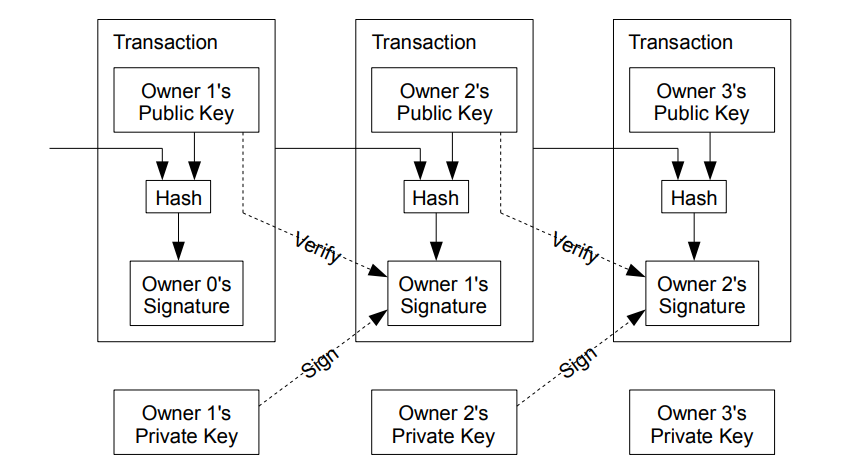
\includegraphics[width=12cm,height=7cm]{Immagini/Transaction_Chain.png}
    \caption[Transaction Chain]{Transazioni memorizzate in un blocco tramite il meccanismo di \textit{Digital Signatures Chain}.}
    \label{transaction_chain}
\end{figure}
Come mostrato in (\ref{struttura_blocco}), all'interno del body di ogni blocco sono presenti diverse transazioni. Queste transazioni sono incluse a loro volta in diverse catene di transazioni; queste ultime permettono di tenere traccia di tutte
le operazioni finanziarie a cui sono stati sottoposti i fondi digitali di tutti i partecipanti. Come affermato nel whitepaper di Bitcoin \cite{bitcoin} ,tutto ciò è definibile come una \textit{moneta digitale}(o elettronica).

\subsection{I Merkle Trees Root e l'integrità dei dati}\label{Merkle_Tree}
Un'altra componente che garantisce l'integrità dei dati presenti in un blocco è il \textit{Merkle Tree}, il quale non è altro che una struttura dati ad \textit{albero}\footnote{Un albero è una struttura dati composta da nodi collegati da archi, creando una gerarchizzazione dei dati presenti al  suo interno.} memorizzata, sotto forma di singola radice (Merkle Tree Root), nell'\textit{header} del blocco(come anticipato in \ref{struttura_blocco}).
Il \textit{bottom layer} di questa struttura ad albero , come viene espresso in un articolo scientifico sul tema \cite{merkle_tree}: “[...] mostra le transazioni memorizzate (ad es. T001 come mostrato in figura \ref{merkle_root_img}) per il blocco, che in seguito vengono convertite nelle loro firme hash SHA256 (ad es. H001 come mostrato in figura \ref{merkle_root_img}) e rappresentano le foglie dell'albero di Merkle.[...]”.

\begin{figure}[h]
    \centering
    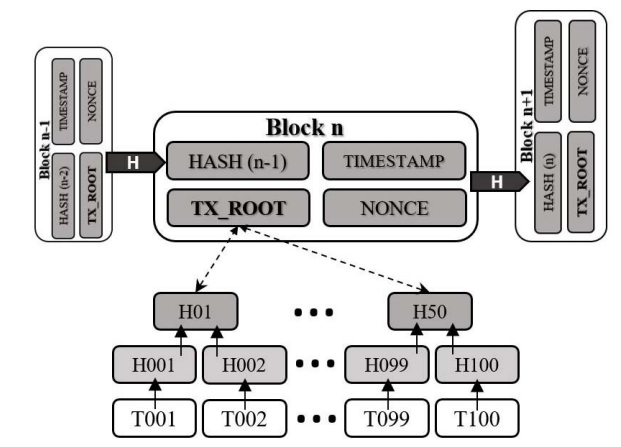
\includegraphics[width=12cm,height=8cm]{Immagini/Merkle_Tree.png}
    \caption[Merkle Tree Root]{Merkle Tree Root memorizzato nell'header di un blocco.}
    \label{merkle_root_img}
\end{figure}
I calcoli della radice di Merkle Tree vengono effettuati attraverso il calcolo dell'hash \textit{ricorsivamente}\footnote{In maniera ricorsiva, ossia espresso in termini di sé stesso.} a partire dalle foglie. Una volta trovato l'hash “finale”, esso rappresenterà la radice del Merkle Tree (definita come TX\_ROOT in figura \ref{merkle_root_img}).

Pertanto, se anche solo un nodo nell'albero venisse modificato, la variazione dei valori hash si diffonderebbe fino alla radice, rendendola immediatamente identificabile. La Merkle Root viene quindi utilizzata per verificare che i blocchi ricevuti dagli altri nodi siano intatti e che nessuna transazione passata sia stata alterata.


\subsection{Il mining per la validazione dei blocchi}\label{mining}
Una volta capito come viene verificata l'autenticità di una transazione, è doveroso sapere come vengono \textit{validate} una o più transazioni. Come anticipato, le transazioni devono essere condivise agli altri nodi della rete (\textit{broadcast}) per essere verificate.
Nel Bitcoin mining , esistono dei \textit{nodi validatori}( i cosidetti \textit{miners}\footnote{I miners sono proprietari di computer che contribuiscono con la loro potenza di calcolo e la loro energia alla rete di una criptovaluta basata sulla Proof-Of-Work}), i quali, una volta ricevute le nuove transazioni attualmente in sospeso, ancora non validate, suggeriscono alla rete quale debba essere il nuovo blocco da pubblicare sul network.
Questi \textit{miners} per validare le transazioni e aggiungerle ad un nuovo blocco, creandolo, devono (come anticipato in \ref{struttura_blocco}) calcolare un valore specifico, chiamato \textit{Nonce}, in maniera tale da soddisfare una particolare proprietà; ricordiamo, inoltre, che ogni valore presente all'interno del blocco che viene modificato, a sua volta modificherà anche il valore hash riferito al blocco stesso.
Il calcolo dei miners che richiede un così grande impegno computazionale è proprio quello di generare uno specifico hash modificando il valore \textit{Nonce} attraverso complessi problemi matematici.

Ogni blocco, dunque, insieme allo storico delle transazioni, dovrà possedere un determinato hash per essere considerato valido a tutti gli effetti ( in Bitcoin, per esempio, il criterio è quello di generare un certo numero di zeri all'inizio del valore hash riferito al blocco). 
Solo i primi minatori che riescono a risolvere il problema vengono ricompensati da una quota di Bitcoin, generata proprio grazie a questo processo.
Ciò significa che coloro i quali possiederanno maggiori risorse computazionali avranno maggiori probabilità di acquisire il “bottino” (block reward \footnote{La ricompensa data ai miners ogni qualvolta viene “minato” un blocco.}) rispetto agli altri. 

Infine, il blocco viene aggiunto alla Blockchain, incrementandone la lunghezza, e le transazioni in esso contenute arrivano a destinazione.
\section{Evoluzione della Blockchain}
In questo capitolo si analizzerà la storia e l'evoluzione di questa tecnologia, si esamineranno tutte le funzionalità che, nel corso degli anni, sono state aggiunte alla Blockchain, partendo dagli albori.

Tratteremo tre diverse varianti:
\begin{itemize}
\item La Blockchain 1.0 : Bitcoin come moneta elettronica peer-to-peer (\ref{Blockchain1.0});
\item La Blockchain 2.0 : Ethereum e l'introduzione agli smart-contract (\ref{Blockchain2.0});
\item La Blockchain 3.0 : Dapp e Blockchain applicata all'industria 4.0 (\ref{Blockchain3.0});
\end{itemize}
\subsection{Blockchain 1.0 : Bitcoin come moneta elettronica peer-to-peer}\label{Blockchain1.0}
Blockchain 1.0 rappresenta la prima applicazione della tecnologia,  implementata da Satoshi Nakamoto, come accennato all'inizio del capitolo \ref{cap1}. 
Questa versione è la configurazione più semplice di registro distribuito (DLT) per la registrazione di transazioni e la memorizzazione dei dati su più computer. La Blockchain di Bitcoin si limita al trasferimento di denaro tra gli utenti senza il bisogno di avere un'autorizzazione esterna(quindi senza intermediazione tra le operazioni finanziarie). Al contempo, le sue caratteristiche (che abbiamo precedentemente conosciuto) ne accentuano il ruolo di potenziale riserva di valore.
\begin{figure}[h]
    \centering
    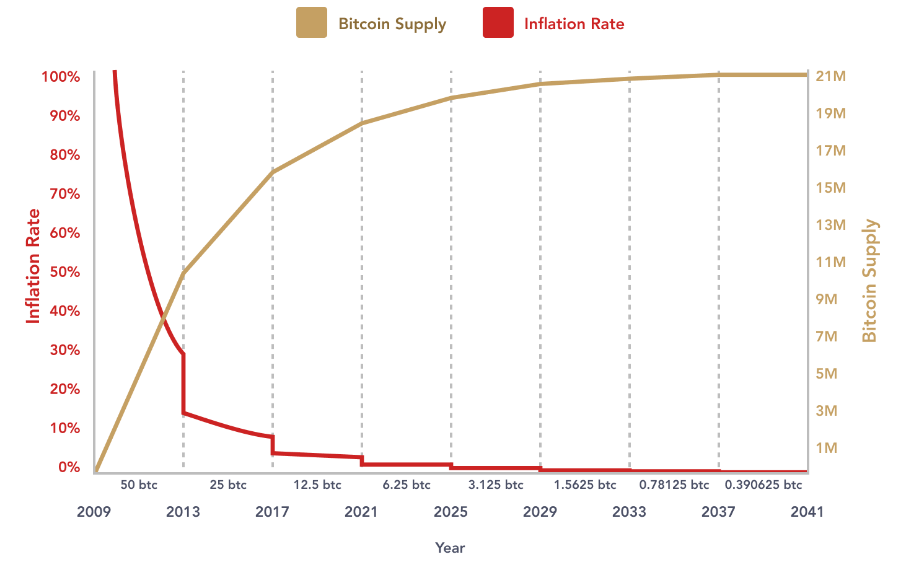
\includegraphics[width=13cm,height=7cm]{Immagini/halving.png}
    \caption[Grafico del tasso inflattivo e della supply di Bitcoin]{Andamento del tasso inflattivo e della \textit{supply} di Bitcoin nel corso del tempo.}
    \label{grafico_inflazione_btc}
\end{figure}
\subsubsection{Come ha fatto Bitcoin a diventare così famoso nel mondo?}
I suoi clamorosi aumenti di valori nel corso della storia e la sua politica monetaria a inflazione\footnote{L'inflazione è il processo in seguito al quale le valute perdono valore nel tempo, causando un aumento dei prezzi dei beni di consumo.} decrescente e \textit{programmata} ha reso famoso Bitcoin facendo parlare di sé e della sua tecnologia in tutto il mondo.
Per capire al meglio come faccia il sistema ad avere una politica deflattiva, introduciamo il concetto di \textit{halving}, ossia quella procedura che dimezza del 50\% la creazione di nuovi Bitcoin ogni 210000 blocchi “minati”(circa ogni 4 anni considerando che il tempo di mining per il singolo blocco è di 10 minuti). La ricompensa iniziale, al momento della pubblicazione di Bitcoin, era di 50 BTC\footnote{Abbreviazione di Bitcoin.} per blocco, ma se questa ricompensa fosse rimasta la stessa, la valuta in circolazione sarebbe aumentata infinitamente nel corso del tempo e si sarebbe verificato, di conseguenza, una continua inflazione. Per evitare questo problema il sistema è stato \textit{programmato} per raggiungere una \textit{max supply}\footnote{La Maximum Supply (offerta totale) di una criptovaluta è la fornitura massima di monete che verranno mai generate.} di 21 milioni di unità.
Il sistema, grazie all'\textit{halving}, quindi, rende Bitcoin più scarso col passare del tempo aumentando il suo prezzo(si evidenzia come Bitcoin sia un asset di natura deflattiva\footnote{Fenomeno opposto all'inflazione, quindi una diminuzione generalizzata dei prezzi, che genera un incremento del potere d'acquisto della moneta.} in figura \ref{grafico_inflazione_btc}). Di seguito si mostra il calcolo per il raggiungimento della \textit{max supply}.
\begin{equation*}
\sum\limits_{i=0}^{32}  210000 \cdot \frac{50}{2^i}       ,dove:
\end{equation*}
\begin{itemize}
\item la variabile \textit{i} rappresenta il numero di \textit{halving} (partendo da zero fino ai 32 \textit{halving} stimati per il futuro);
\item \textit{210000} sono i numeri di blocchi da minare (il processo di mining viene spiegato in \ref{mining}) per fare in modo che si passi all'\textit{halving} successivo e si incrementi la variabile i;
\item il valore \textit{50} corrisponde, come anticipato, alla ricompensa iniziale di BTC per ogni blocco minato. Quest'ultimo viene diviso per \textit{$2^i$} volte.
\end{itemize}

Logicamente, una ricompensa sempre più bassa comporta meno generazione di moneta e di conseguenza un maggior tempo per raggiungere la \textit{max supply}, di fatto, la data stimata in cui verrà raggiunta si aggira intorno al 2140.

Possiamo sintetizzare la prima generazione di Blockchain come l'innesco che ha dato il via alla rivoluzione degli scambi peer-to-peer monetari. L'interesse mondiale verso Bitcoin ha posto le basi per lo studio di nuovi possibili sviluppi e use-case per questa tecnologia.
\subsection{ Blockchain 2.0 : Ethereum e la programmabilità della Blockchain tramite smart-contract (DeFi e Dapp)}\label{Blockchain2.0}
La seconda generazione di Blockchain è rappresentata da Ethereum\footnote{Da: \cite{ethereum_definizione} “Ethereum è una piattaforma decentralizzata del Web 3.0 per la creazione e pubblicazione peer-to-peer di contratti intelligenti[...]. La criptovaluta legata ad essa è Ether. Descritta per la prima volta in \cite{ethereum}.} \cite{ethereum}.
Dopo il rilascio di Bitcoin, la Blockchain ha conquistato rapidamente la fantasia degli sviluppatori di tutto il mondo. Nel 2013 (circa 4 anni dopo l'ascesa di Bitcoin) un ragazzo di appena 19 anni di nome Vitalik Buterin\footnote{Sviluppatore di origini russe, ideatore di Ethereum.} propone ad un team di sviluppatori un whitepaper. Dopo aver approvato la sua idea, questi sviluppatori cominciano a lavorare insieme a Vitalik per definire gli ultimi dettagli. L'anno successivo (nel 2014) viene presentato ufficialmente alla North American Bitcoin Conference a Miami il whitepaper finale di Ethereum \cite{ethereum}, rivoluzionando la visione di questa tecnologia nel mondo.

L'idea alla base di Ethereum è quella di creare un grande sistema decentralizzato, che vada oltre il fatto di essere un semplice mezzo di pagamento o un modo per trasferire denaro, e che renda la sua struttura programmabile in toto, dall'automatizzazione degli scambi monetari a veri e propri applicativi decentralizzati.

Per rendere tutto questo possibile, sono stati introdotti gli \textit{smart-contract}(o contratti intelligenti): programmi informatici o codici archiviati nella Blockchain che vengono eseguiti quando vengono soddisfatte condizioni predeterminate.
In Ethereum gli  \textit{smart-contract} sono scritti in Solidity(linguaggio di programmazione approfondito al capitolo \ref{cap2}), uno degli strumenti cardine per lo sviluppo dell'applicazione che verrà mostrata in questo elaborato. 

Il codice degli \textit{smart-contract} viene eseguito in un ambiente chiamato \textit{Ethereum Virtual Machine} (EVM), utilizzato da Ethereum, oltre che per rendere possibile la corretta esecuzione dei codici, anche per implementare tutte quelle funzionalità aggiuntive in maniera tale da mettere in piedi un ecosistema vero e proprio.


In una famosa pubblicazione di \textit{Apress}, nella quale viene introdotto lo studio di Ethereum e della programmazione smart-contract \cite{EthereumBook}, viene affermato quanto segue:“Ethereum cerca di creare un sistema in cui i modelli economici possono essere provati e dimostrati. Per il momento, Solidity sembra destinato a diventare il linguaggio de facto di tali modelli, a condizione che vengano eseguiti su una macchina virtuale globale come l'EVM.”.

Di fatto, riconosce il potenziale di Solidity e degli \textit{smart-contract}, i quali, venendo eseguiti in ambiente Blockchain, ne ereditano tutti i vantaggi, tra cui:

\begin{itemize}
\item Sicurezza:La Blockchain in cui viene registrato il codice informatico del contratto intelligente non consente di essere manomesso e garantisce che possa essere eseguito in modo affidabile,generando risultati sempre verificabili e immutabili;
\item Trasparenza: I record crittografati delle transazioni sono condivisi tra i partecipanti;
\item Risparmio: I contratti intelligenti eliminano la necessità per gli intermediari di gestire le transazioni e, per estensione, i ritardi e le commissioni associati.
\end{itemize}

I contratti intelligenti consentono a due parti di eseguire automaticamente attività molto complesse facilitando lo scambio di valuta digitale, ereditando tutti i vantaggi della Blockchain.

In definitiva, la Blockchain 2.0 ha aperto le porte ad un'infinità di possibili implementazioni e applicazioni.
Tra le più importanti ricordiamo la DeFi, argomento vertice dell'elaborato, spiegato di seguito.

\subsubsection{Decentralized Finance (o DeFi)} 
La \textit{Decentralized Finance} (o DeFi) è uno degli argomenti più discussi nelle comunità Blockchain; essa propone di disintermediare modelli finanziari tradizionali eliminando entità centrali(come banche, istituti di credito, ecc...) dando la possibilità di erogare ed usufruire di servizi finanziari in maniera del tutto decentralizzata. Questi servizi finanziari vengono erogati dalle {Decentralized Application}\footnote{Applicazioni che hanno il proprio codice di back-end in esecuzione su una rete peer-to-peer decentralizzata e ciò la differenzia della maggior parte delle comuni applicazioni il cui codice di back-end è in esecuzione su server centralizzati.} (o Dapp) , ossia delle web-application basate su reti P2P che sfruttano le potenzialità della Blockchain.

Come le normali applicazioni, le Dapp sono composte da un front-end\footnote{La parte visibile all'utente di un programma e con cui egli può interagire.}, un back-end\footnote{La parte non visibile all'utente di un programma che gestisce le funzioni dell'applicazione “dietro le quinte”.} e da un database (in questi casi è la Blockchain o gli smart-contract a fare da database).
La particolarità di queste applicazioni è che, sfruttando la Blockchain, i dati inseriti dagli utenti vengono memorizzati su un registro distribuito in maniera del tutto automatica, grazie all'utilizzo degli \textit{smart-contract} precedentemente introdotti.

Le applicazioni DeFi sono divisi il 5 livelli distinti, come definito in \cite{DeFi_article}:
\begin{itemize} 
 \item Il primo livello è il \textit{settlement layer} (o livello dei regolamenti) in cui vengono regolate tutte le transazioni. Su questo livello si trova la Blockchain e il suo relativo asset nativo ( ad esempio, Ether per la Blockchain di Ethereum).
 La Blockchain, come si dice in \cite{DeFi_article}:“può essere vista come la base per l'esecuzione senza fiducia e serve come livello di risoluzione delle controversie.”;
 \item Il secondo livello è l'\textit{asset layer}. In questo livello sono presenti tutti gli asset emessi dal livello di regolamento, solitamente indicati come token, fungibili\footnote{Un token si dice fungibile quando può essere duplicato un numero infinito di volte in copie identiche e intercambiabili.} e non fungibili come gli NFT(acronimo di Not-Fungible-Token ,anche chiamati “certificati digitali”, da \cite{NFT_definizione} sono: “asset crittografici su una Blockchain con codici di identificazione e metadati unici che li distinguono gli uni dagli altri. Essi non possono essere scambiati in modo equivalente.”);
 
 \item Il terzo livello è il \textit{protocol layer} (o livello dei protocolli), tale livello contiene un insieme di regole e standard concordati che normano le transazioni. Queste regole e standard sono implementati da una serie di \textit{smart-contract};
 \item Il quarto livello è l'\textit{application layer} (o livello di applicazione), il livello nel quale si posiziona l'applicazione implementata per questo elaborato.
 Di fatto, l'\textit{application layer} crea applicazioni che si collegano ai protocolli tramite l'\textit{interazione agli smart-contract}, rendendo i protocolli molto più facili da usare;
 \item Il quinto livello, infine, è l'\textit{aggregation layer} (o livello di aggragazione) il quale fornisce strumenti per la comparazione e la valutazione dei servizi, consentendo agli utenti di svolgere attività altrimenti complesse.
 \end{itemize}

Si mostra in figura \ref{defi_img} una rappresentazione grafica della struttura di un'applicazione DeFi. 

\begin{figure}[h]
    \centering
    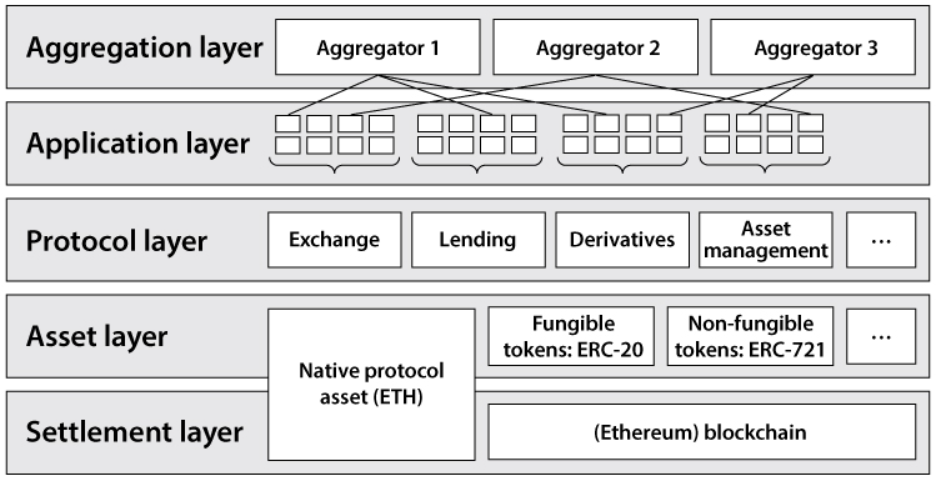
\includegraphics[width=12cm,height=8cm]{Immagini/Defi.png}
    \caption{Struttura di un'applicazione DeFi.}
    \label{defi_img}
    \label{fig:The DeFi Stack}
\end{figure}
\subsection{Blockchain 3.0 : Blockchain applicata all'industria 4.0}\label{Blockchain3.0}
Gli sviluppi successivi alla Blockchain 2.0 non hanno una definizione molto chiara, trattandosi di argomenti in continuo sviluppo.
Oggi come oggi, potremmo comunque definire la Blockchain 3.0 come quell'ondata evolutiva che cerca di oltrepassare e ottimizzare i servizi delle prime due generazioni, rendendo, al contempo, la tecnologia Blockchain utilizzabile per le esigenze aziendali.
Sopratutto riferiti all'industria 4.0, la quale, in breve, non è altro che, come viene detto in \cite{industria4.0}:“la propensione dell'odierna automazione industriale ad inserire alcune nuove tecnologie produttive per migliorare le condizioni di lavoro, creare nuovi modelli di business, aumentare la produttività degli impianti e migliorare la qualità dei prodotti. [...]”.
Questa particolare rivoluzione industriale richiede (come d'altronde in generale nel prossimo futuro) un grado sempre più alto di sicurezza della privacy e dei dati e maggiore fiducia. Qui entra in gioco la Blockchain.

Le principali preoccupazioni per questa generazione di Blockchain sono la sostenibilità, la scalabilità, l'economicità, una maggiore decentralizzazione e una maggiore sicurezza.

La sostenibilità, che è un argomento di forte attualità, influenza le scelte delle nuove famiglie di Blockchain. Molte Blockchain, come è stato già anticipato nei capitoli precedenti, necessitano di grandi potenze di calcolo per alcune operazioni ( si pensi, per esempio, al mining) comportando un grande dispendio energetico. Non a caso le Blockchain si stanno aggiornando tenendo in considerazione questo fattore( basti guardare al Merge di Ethereum \cite{TheMerge}), passando a modelli più sostenibili come il Proof-Of-Stake (PoS).

%La Blockchain 3.0 ,inoltre, deve essere capace di integrare e supportare altri contesti applicativi come quelli dell'\textit{Internet of Things}\footnote{Da \cite{IoT} :”neologismo utilizzato nel mondo delle telecomunicazioni e dell'informatica che fa riferimento all'estensione di internet al mondo degli oggetti e dei luoghi concreti, che acquisiscono una propria identità digitale in modo da poter comunicare con altri oggetti nella rete e poter fornire servizi agli utenti.”}(Iot) o dell' \textit{Intelligenza Artificiale}\footnote{L'intelligenza artificiale, anche chiamata IA, come detto in \cite{IA} è :”una disciplina che studia se e in che modo si possano realizzare sistemi informatici intelligenti in grado di simulare la capacità e il comportamento del pensiero umano.[...]”}, puntando sempre di più sulle Dapp.


In conclusione, al netto di tutti questi incredibili possibili sviluppi, la tecnologia Blockchain ha ancora molto da offrire al mondo che verrà, rendendola, di fatto, una delle tecnologie più interessanti da approfondire.